\documentclass{exam}
\usepackage[top=.4in, bottom=.1in, left=1in, right=.4in]{geometry}
\textheight=6in
\usepackage{tikz}

\begin{document}

\pagenumbering{gobble}
\newgeometry{bottom=0.1cm}

\begin{center}
\fbox{\fbox{\parbox{5.5in}{\centering
Answer the questions here as you wish - circle/underline correct choices. Be careful there are open-typed questions. In the spaces provided write your answers. If you run out of room
for an answer, continue on the back of the page.}}}
\end{center}

\vspace{5mm}

\makebox[\textwidth]{Name and section:\enspace\hrulefill}

\vspace{5mm}

\makebox[\textwidth]{Instructor's name:\enspace\hrulefill}
\vspace{5mm}

\begin{questions}

\question Who is the Steve Jobs?

\begin{oneparchoices}
\choice Apple CEO
\choice Dead man
\choice Legend
\end{oneparchoices} %question1

\question test2

\begin{solutionorlines}[0.5in]
\end{solutionorlines}%question2

\question test3

\begin{oneparchoices}
\choice c
\choice c
\choice c
\choice c
\choice c
\end{oneparchoices} %question3

\end{questions}

\newpage

\begin{center}
    \textbf{\Large OMR answer sheet for Test}
\end{center}

\begin{flushright}
    Date:
    \begin{tabular}{|c|c|c|c|c|c|c|c|} \hline
         & & & & & & & & \hline
    \end{tabular} \\
\end{flushright}

\begin{flushleft}
  \vspace{1em}
    Number of ID:
        \begin{tabular}{|c|c|c|c|c|} \hline
         & & & & &\hline
    \end{tabular} \\
\end{flushleft}

\tikzstyle{green}=[fill=red!0]
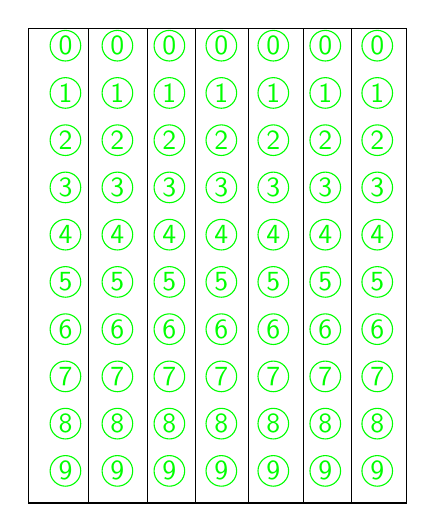
\begin{tikzpicture}[font={\sffamily},x=2cm]
\begin{scope}[xshift=0 cm]
		\begin{scope}[yshift=-12,xshift=3.2]
				\foreach \digit in {0,1,2,3,4,5,6,7,8,9} {
						\begin{scope}[yshift=-.6*\digit cm]
								\foreach \count/\desc in {1/0, 2/0, 3/0, 4/0, 5/0, 6/0, 7/0} {
								\node[green,draw,circle,inner sep=1pt] at ({\count * 0.33},-.05) {\digit};
								 }
						 \end{scope}
		}
		\end{scope}
		\draw (.15,-.25) rectangle(2.55,-6.28);
		\draw (2.20,-.25) rectangle(2.55,-6.28);
		\draw (1.90,-.25) rectangle(2.55,-6.28);
		\draw (1.55,-.25) rectangle(2.55,-6.28);
		\draw (1.21,-.25) rectangle(2.55,-6.28);
		\draw (0.91,-.25) rectangle(2.55,-6.28);
		\draw (0.53,-.25) rectangle(2.55,-6.28);
\end{scope}


\end{tikzpicture}

\vspace{.4em}
\hrule
\vspace{1em}

\begin{center}
\begin{tabular}{|l|}
		\hline
{INSTRUCTIONS}  \\
    \hline
1.  Use HB pencil or black pen only this sheet.  \\
2.  Darken the ovals fully.  \\
3.  Do not make any stray marks on this sheet.\\
4.  Don't user eraser to correct darkened circles.\\
    \hline
\end{tabular}
\end{center}

    \vspace{1em}
        \hrule

\begin{tikzpicture}[font={\sffamily},overlay]

%begin answer1
\begin{scope}[yshift=-1.5cm]
		\draw(-.22,-.35) rectangle(10cm,.9em);
		\pgfmathtruncatemacro\q{(1)}
		\node at (0,-.05) {\normalsize{\q}};
				\foreach \count/\desc in {1/A, 2/B, 3/C, 4/D, 5/E} {
						\node[draw,circle,inner sep=1pt] at ({\count+1 * 0.5},-.05) {\desc};
				}
\end{scope} %new_answer_here1



%begin_answer2
\begin{scope}[yshift=-2.5cm]
        \draw(-.22,-.35) rectangle(10cm,.9em);
        \pgfmathtruncatemacro\q{(2)}
        \node at (0,-.05) {\normalsize{\q}};
\end{scope}

\begin{scope}[yshift=-2.5cm, xshift=13cm]
        \draw(-.22,-.35) rectangle(2cm,.9em);
        \node at (0,-.05) {\normalsize{\q}};
\end{scope} %new_answer_here2

%begin_answer3
\begin{scope}[yshift=-3.5cm]
		\draw(-.22,-.35) rectangle(10cm,.9em);
		\pgfmathtruncatemacro\q{(3)}
		\node at (0,-.05) {\normalsize{\q}};
				\foreach \count/\desc in {1/A, 2/B, 3/C, 4/D, 5/E} {
						\node[draw,circle,inner sep=1pt] at ({\count+1 * 0.5},-.05) {\desc};
				}
\end{scope} %new_answer_here3




\end{tikzpicture}
\end{document}
